%! TeX root = Downloads/Berkeley/Math/Math128a/Homework/Math128aHw11/Math128aHw11.tex

\documentclass{article}
\usepackage{/Users/trustinnguyen/.mystyle/math/packages/mypackages}
\usepackage{/Users/trustinnguyen/.mystyle/math/commands/mycommands}
\usepackage{/Users/trustinnguyen/.mystyle/math/environments/article}
\graphicspath{{./figures/}}

\title{Math128aHw11}
\author{Trustin Nguyen}

\begin{document}

    \maketitle

\reversemarginpar

\section*{Exercise Set 5.9}

\textbf{Exercise 2}: Use the Runge-Kutta method for systems to approximate the solutions of the following systems of first-order differential equations and compare the results to the actual solutions.
    \begin{itemize}
        \item [b]. 
            \begin{align*}
                u_{1}^{\prime} &= \dfrac{1}{9}u_{1} - \dfrac{2}{3}u_{2} - \dfrac{1}{9}t^{2} + \dfrac{2}{3} \\
                u_{2}^{\prime} &= u_{2} + 3t - 4                                                           \\
                u_{1}(0)       &= -3                                                                       \\
                u_{2}(0)       &= 5                                                                          
            \end{align*}
        for $0 \leq t \leq 2$, $h = 0.2$.
    \end{itemize}
    \begin{answer}
        Here is the comparison:
            \begin{center}
                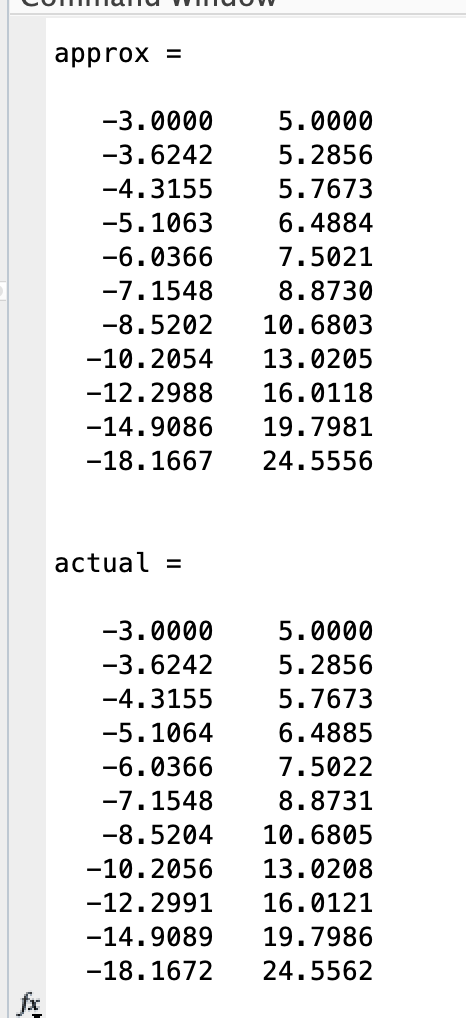
\includegraphics[scale=0.5]{q1}
            \end{center}
        and here is my code:
        \inputminted{matlab}{./code/RKsystem.m}
        \inputminted{matlab}{./code/q1f1.m}
        \inputminted{matlab}{./code/q1f2.m}
        \inputminted{matlab}{./code/q1actf1.m}
        \inputminted{matlab}{./code/q1actf2.m}
        \inputminted{matlab}{./code/evalAct.m}
        \inputminted{matlab}{./code/script1.m}
    \end{answer}

\textbf{Exercise 4}: Use the Runge-Kutta for Systems Algorithm to approximate the solutions of the following higher-order differential equations and compare the results to the actual solutions.
    \begin{itemize}
        \item [b] $t^{2}y^{\prime\prime} + ty^{\prime} - 4y = -3t, 1 \leq t \leq 3, y(1) = 4, y^{\prime}(1) = 3$, with $h = 0.2$; actual solution $y(t) = 2t^{2} + t + t^{-2}$.
    \end{itemize}
    \begin{answer}
        Let 
            \begin{equation*}
                u_{1} = y, u_{2} = y^{\prime}
            \end{equation*}
        Then we get:
            \begin{equation*}
                u_{1}^{\prime} = u_{2}
            \end{equation*}
        and
            \begin{equation*}
                t^{2}u_{2}^{\prime} + tu_{2} - 4u_{1} = -3t
            \end{equation*}
        so
            \begin{equation*}
                u_{2}^{\prime} = \dfrac{1}{t^{2}}(-tu_{2} + 4u_{1} -3t)
            \end{equation*}
        Now we apply RK with 
            \begin{align*}
                u_{1}^{\prime} &= u_{2}                                                    \\
                u_{2}^{\prime} &= \dfrac{4}{t^{2}}u_{1} - \dfrac{1}{t}u_{2} - \dfrac{3}{t} \\
                u_{1}(1)       &= 4                                                        \\
                u_{2}(1)       &= 3                                                          
            \end{align*}
        Here is my comparison:
            \begin{center}
                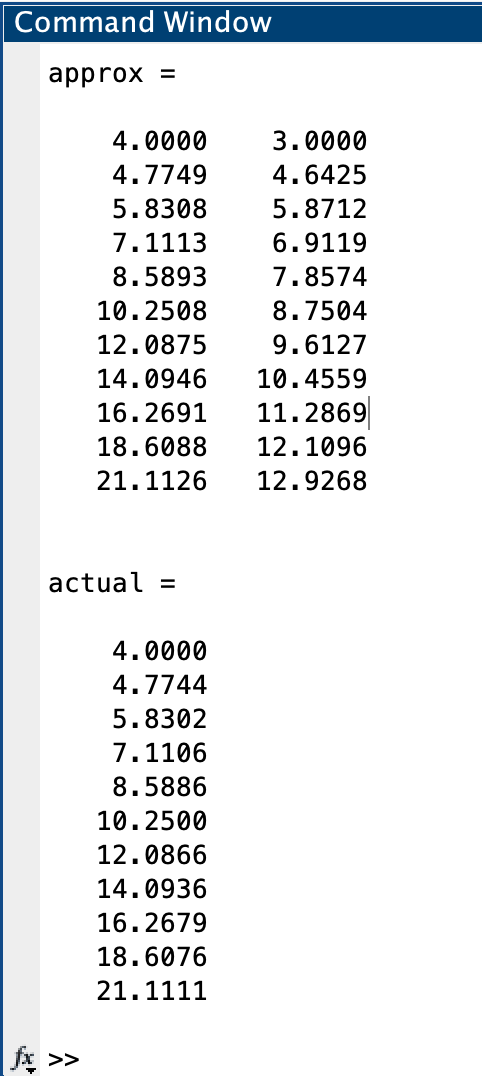
\includegraphics[scale=0.5]{q2}
            \end{center}
        and my code:
        \inputminted{matlab}{./code/RKsystem.m}
        \inputminted{matlab}{./code/q2f1.m}
        \inputminted{matlab}{./code/q2f2.m}
        \inputminted{matlab}{./code/q2actf1.m}
        \inputminted{matlab}{./code/evalAct.m}
        \inputminted{matlab}{./code/script2.m}
    \end{answer}

\textbf{Exercise 5}: The study of mathematical models for predicting the population dynamics of competing species has its origin in independent works published in the early part of the 20th century by A. J. Lotka and V. Volterra (see, for example, |Lol |, rLo21, and |Vo|.).

Consider the problem of predicting the population of two species, one of which is a predator, whose population at time $t$ is $x_{2}(t)$, feeding on the other, which is the prey, whose population is $x(t)$. We will assume that the prey always has an adequate food supply and that its birthrate at any time is proportional to the number of prey alive at that time; that is, birthrate (prey) is $k_{1}x_{1}(t)$. The death rate of the prey depends on both the number of prey and predators alive at that time. For simplicity, we assume death rate (prey) = $k_{2}x_{1}(t)x_{2}(t)$. The birthrate of the predator, on the other hand, depends on its food supply, $x(t)$ as well as on the number of predators available for reproduction purposes. For this reason, we assume that the birthrate (predator) is $k_{3}x(t)x_{2}(t)$. The death rate of the predator will be taken as simply proportional to the number of predators alive at the time; that is, death rate (predator) = $k_{4}x_{2}(t)$.

Since $x(t)$ and $x_{2}(t)$ represent the change in the prey and predator populations, respectively, with respect to time, the problem is expressed by the system of nonlinear differential equations
    \begin{equation*}
        x^{\prime}_{1}(t) = k_{1}x_{1}(t) - k_{2}x_{1}(t)x_{2}(t) \hspace{30pt}  \text{ and } \hspace{30pt}  x_{2}^{\prime}(t) = k_{3}x_{1}(t)x_{2}(t) - k_{4}x_{2}(t)
    \end{equation*}
    Solve this system for $0 < t < 4$, assuming that the initial population of the prey is $1000$ and of the predators is $500$ and that the constants are $k_{1} = 3, k_{2} = 0.002, k_{3} = 0.0006$, and $k_{4} = 0.5$. Sketch a graph of the solutions to this problem, plotting both populations with time, and describe the physical phenomena represented. Is there a stable solution to this population model? If so, for what values $x_{1}$ and $x_{2}$ is the solution stable?
    \begin{answer}
        Here is the graph:
            \begin{center}
                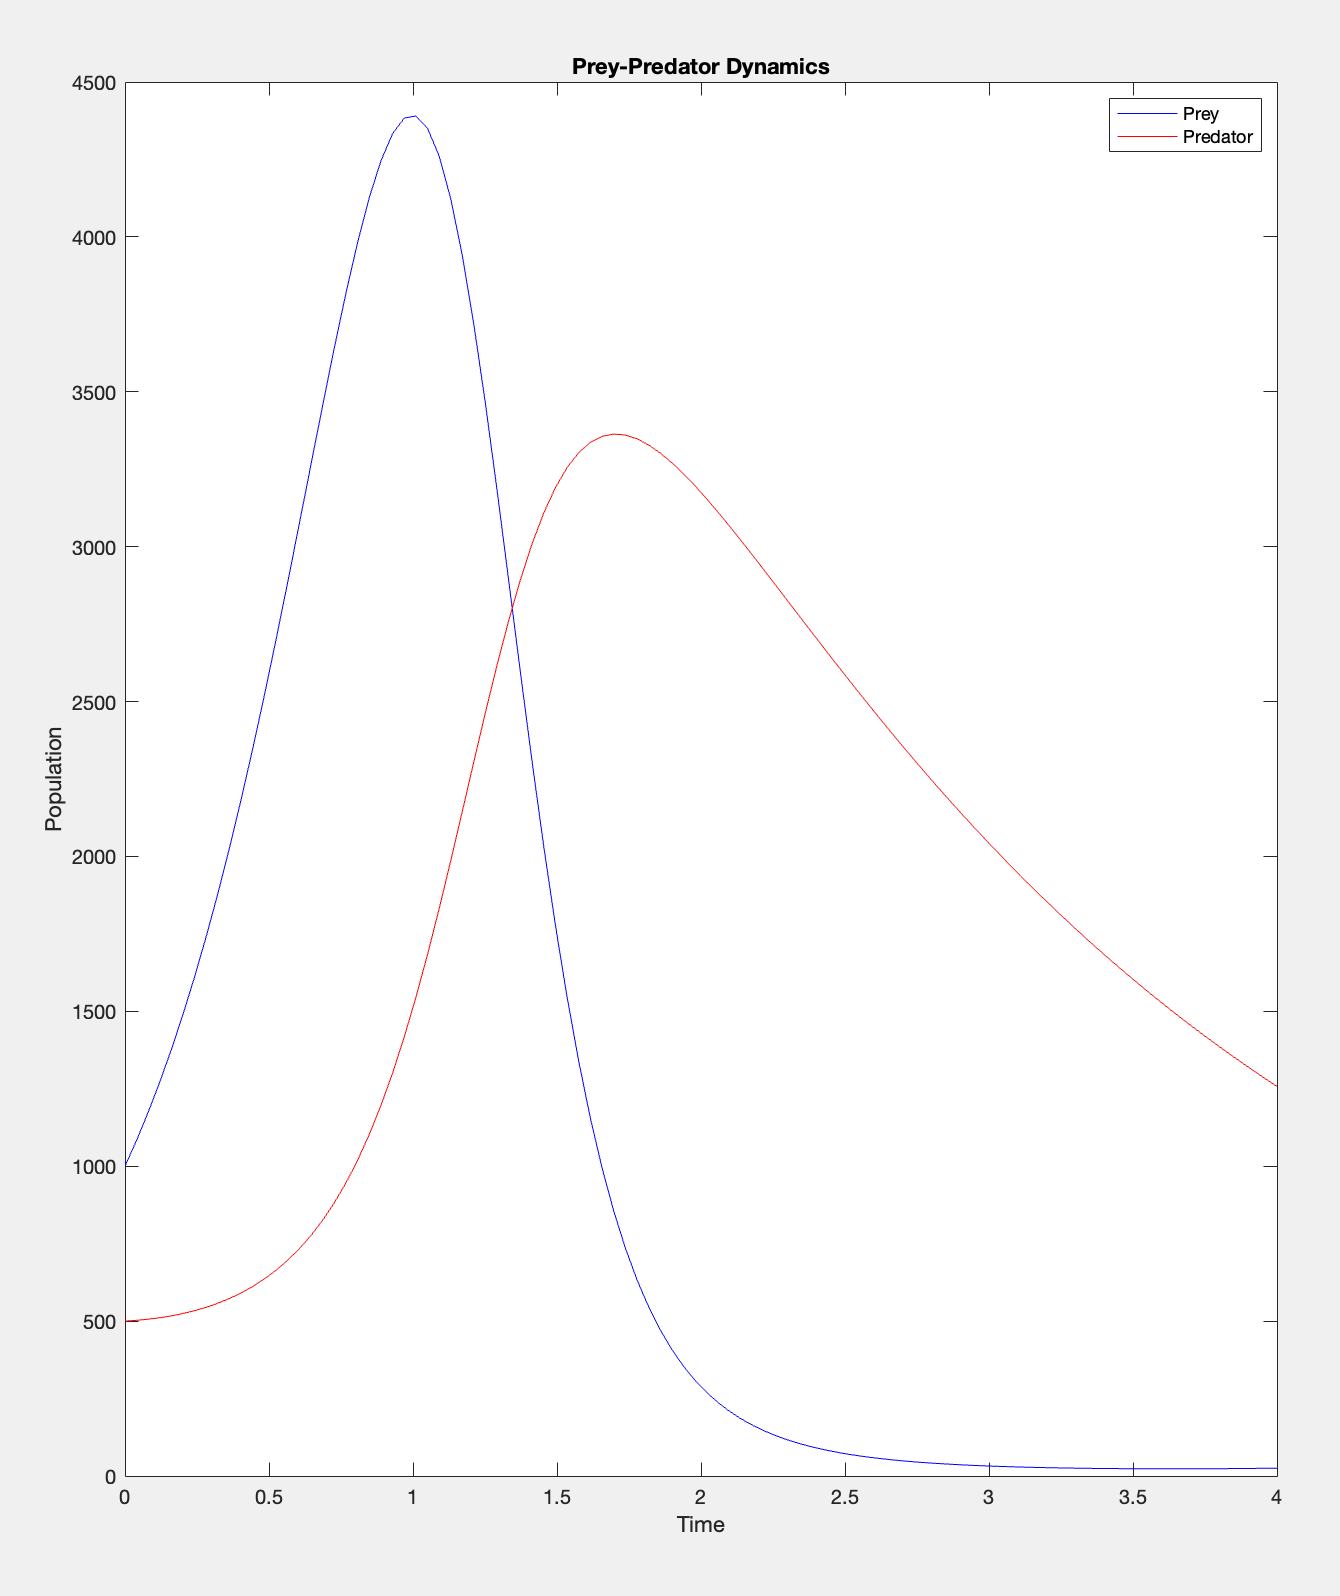
\includegraphics[scale=0.5]{q3}
            \end{center}
        and here is my code:
        \inputminted{matlab}{./code/RKsystem.m}
        \inputminted{matlab}{./code/q3f1.m}
        \inputminted{matlab}{./code/q3f2.m}
        \inputminted{matlab}{./code/script3.m}
    \end{answer}

\textbf{Exercise 6}: In Exercise 5, we considered the problem of predicting the population in a predator-prey model. Another problem of this type is concerned with two species competing for the same food supply. If the numbers of species alive at time $t$ are denoted by $x_{1}(t)$ and $x_{2}(t)$, it is often assumed that, although the birthrate of each of the species is simply proportional to the number of species alive at that time, the death rate of each species depends on the population of both species. We will assume that the population of a particular pair of species is described by the equations
    \begin{align*}
        \dv{x_{1}(t)}{t} &= x_{1}(t)[4 - 0.0003x_{1}(t) - 0.0004 x_{2}(t)]  \\
        \dv{x_{2}(t)}{t} &= x_{2}(t)[2 - 0.0002 x_{1}(t) - 0.0001 x_{2}(t)]   
    \end{align*}
If it is known that the initial population of each species is $10,000$, find the solution to this system for $0 < t < 4$. Is there a stable solution to this population model? If so, for what values of $x_{1}$ and $x_{2}$ is the solution stable?
    \begin{answer}
        Here is my graph:
        \begin{center}
            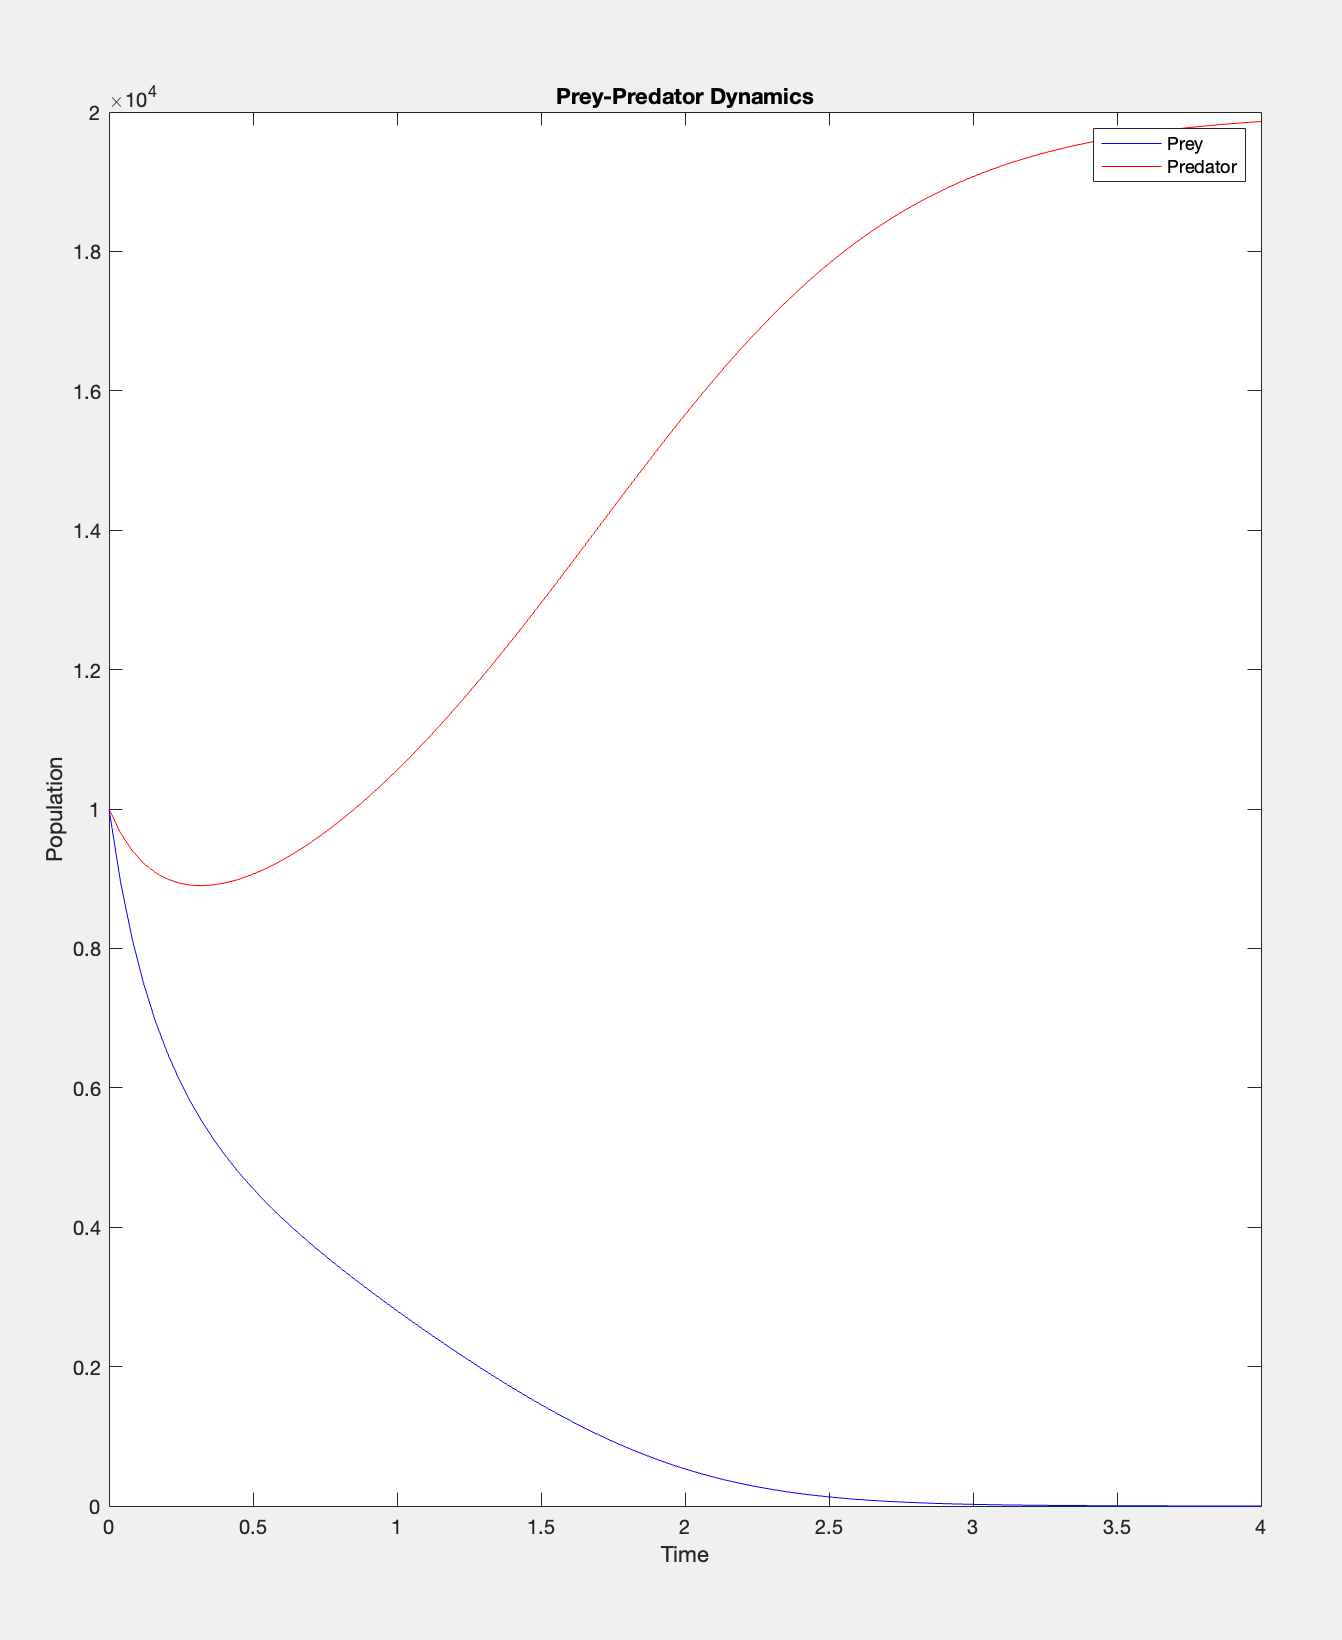
\includegraphics[scale=0.5]{q4}
        \end{center}
        and the code:
        \inputminted{matlab}{./code/RKsystem.m}
        \inputminted{matlab}{./code/q4f1.m}
        \inputminted{matlab}{./code/q4f2.m}
        \inputminted{matlab}{./code/script4.m}
    \end{answer}

\newpage
\section*{Exercise Set 5.11}
\hrule

\textbf{Exercise 2}: Solve the following stiff initial-value problems using Euler's method and compare the results with the actual solution.
    \begin{itemize}
        \item [b] $y^{\prime} = -10y + 10t + 1, 0 \leq t \leq 1, y(0) = e$, with $h  = 0.1$; actual solution $y(t) = e^{-10t + 1} + t$.
    \end{itemize}
    \begin{answer}
        Here are the approximations vs the actual result:
        \begin{center}
            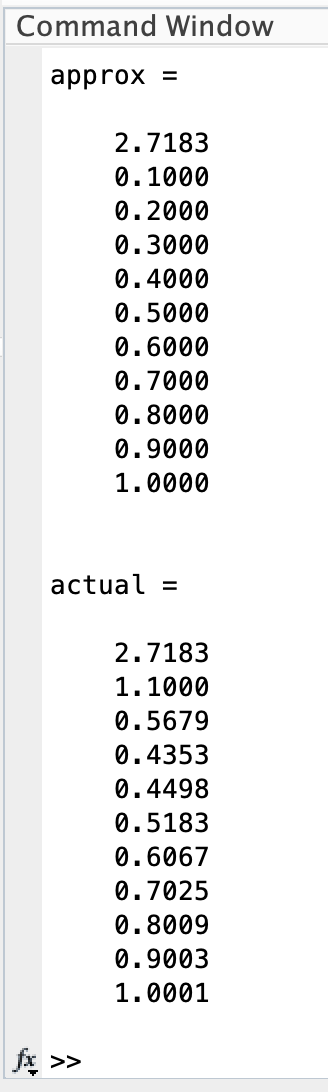
\includegraphics[scale=0.5]{q5}
        \end{center}
        And here is my code:
        \inputminted{matlab}{./code/Euler.m}
        \inputminted{matlab}{./code/q5f.m}
        \inputminted{matlab}{./code/q5actf.m}
        \inputminted{matlab}{./code/evalActStiff.m}
        \inputminted{matlab}{./code/script6.m}
    \end{answer}

\textbf{Exercise 4}: Repeat Exercise 2 using the Runge-Kutta fourth-order method.
    \begin{itemize}
        \item [b] $y^{\prime} = -10y + 10t + 1, 0 \leq t \leq 1, y(0) = e$, with $h  = 0.1$; actual solution $y(t) = e^{-10t + 1} + t$.
    \end{itemize}
    \begin{answer}
        Here are the approximations vs the actual result:
        \begin{center}
            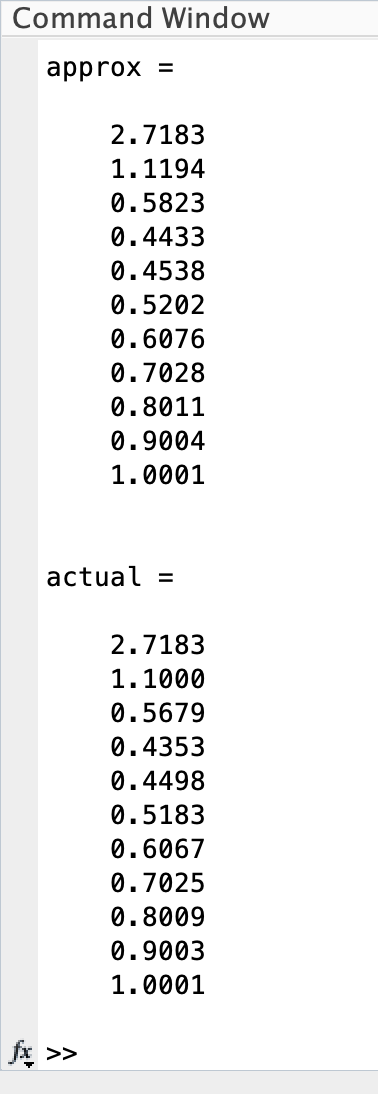
\includegraphics[scale=0.5]{q6}
        \end{center}
        and here is my code:
        \inputminted{matlab}{./code/RKfourth.m}
        \inputminted{matlab}{./code/q5f.m}
        \inputminted{matlab}{./code/q5actf.m}
        \inputminted{matlab}{./code/evalActStiff.m}
        \inputminted{matlab}{./code/script7.m}
    \end{answer}

\textbf{Exercise 8}: Repeat Exercise $2$ using the Trapezoidal Algorithm with $TOL = 10^{-5}$.
    \begin{itemize}
        \item [b] $y^{\prime} = -10y + 10t + 1, 0 \leq t \leq 1, y(0) = e$, with $h  = 0.1$; actual solution $y(t) = e^{-10t + 1} + t$.
    \end{itemize}
    \begin{answer}
        Here are the approximations vs the actual result:
        \begin{center}
            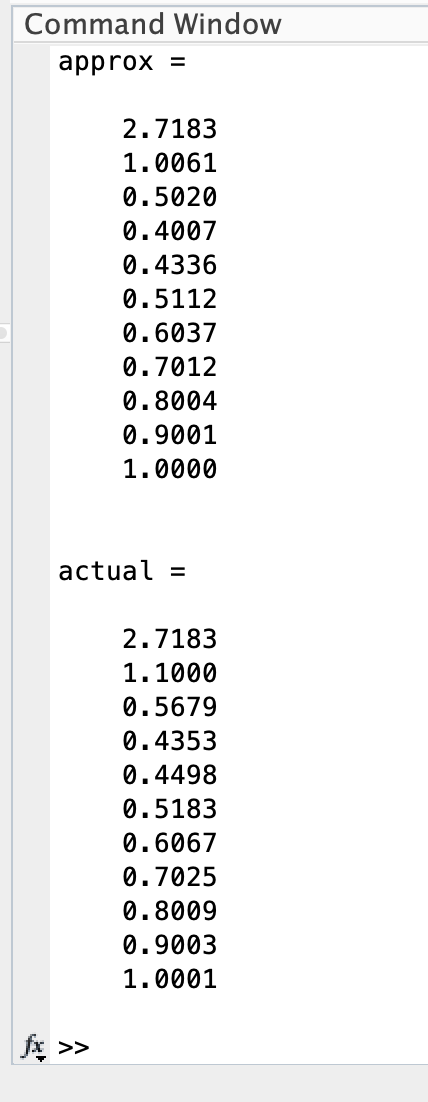
\includegraphics[scale=0.5]{q7}
        \end{center}
        and here is my code:
        \inputminted{matlab}{./code/TrapezoidNewton.m}
        \inputminted{matlab}{./code/q5f.m}
        \inputminted{matlab}{./code/q5fdy.m}
        \inputminted{matlab}{./code/q5actf.m}
        \inputminted{matlab}{./code/evalActStiff.m}
        \inputminted{matlab}{./code/script8.m}
    \end{answer}

\textbf{Exercise 10}: Show that the fourth-order Runge-Kutta method
    \begin{align*}
        k_{1}     &= hf(t_{i}, w_{i})                              \\
        k_{2}     &= hf(t_{i} + h / 2, w_{i} + k_{1} / 2)          \\
        k_{3}     &= hf(t_{i} + h / 2, w_{i} + k_{2} / 2)          \\
        k_{4}     &= hf(t_{i} + h, w_{i} + k_{3})                  \\
        w_{i + 1} &= w_{i} + (k_{1} + 2k_{2} + 2k_{3} + k_{4}) / 6   
    \end{align*}
when applied to the differential equation $y^{\prime} = \lambda y$, can be written in the form
    \begin{equation*}
        w_{i + 1} = \left(1 + h\lambda + \dfrac{1}{2}(h\lambda)^{2} + \dfrac{1}{6}(h\lambda)^{3} + \dfrac{1}{2}(h\lambda)^{4}\right)
    \end{equation*}
    \begin{answer}
        We evaluate:
            \begin{align*}
                k_{1} &= hw_{i}\lambda               \\
                k_{2} &= h(w_{i} + k_{1} / 2)\lambda \\
                k_{3} &= h(w_{i} + k_{2} / 2)\lambda \\
                k_{4} &= h(w_{i} + k_{3})\lambda       
            \end{align*}
        then
            \begin{equation*}
                k_{2} = hw_{i}(1 + h\lambda / 2)\lambda = w_{i}(h\lambda + (h\lambda)^{2} / 2)
            \end{equation*}
        and
            \begin{equation*}
                k_{3} = hw_{i}(1 + h(1 + h\lambda/2)\lambda/2)\lambda = hw_{i}(1 + h\lambda/2 + h^{2}\lambda^{2}/4)\lambda = w_{i}(h\lambda + (h\lambda)^{2} / 2 + (h\lambda)^{3}/4)
            \end{equation*}
        and
            \begin{equation*}
                k_{4} = hw_{i}(1 + h\lambda / 2+ (h\lambda)^{2} / 4 + (h\lambda)^{3} / 8)\lambda = w_{i}(h\lambda + (h\lambda)^{2} / 2 +  (h\lambda)^{3} / 4 + (h\lambda)^{4} / 8)
            \end{equation*}
        now
            \begin{equation*}
                2k_{2} = w_{i}(2h\lambda + (h\lambda)^{2})
            \end{equation*}
        and
            \begin{equation*}
                2k_{3} = w_{i}(2h\lambda + (h\lambda)^{2} + (h\lambda)^{3} / 2)
            \end{equation*}
        now add then together:
            \begin{align*}
                k_{1}  &= w_{i}h\lambda                                                                \\
                2k_{2} &= w_{i}(2h\lambda + (h\lambda)^{2})                                            \\
                2k_{3} &= w_{i}(2h\lambda + (h\lambda)^{2} + (h\lambda)^{3} / 2)                       \\
                k_{4}  &= w_{i}(h\lambda + (h\lambda)^{2} /2 + (h\lambda)^{3} / 4 + (h\lambda)^{4}/8)    
            \end{align*}
        we get
            \begin{equation*}
                w_{i + 1} = \left(1 + h\lambda + \dfrac{1}{2}(h\lambda)^{2} + \dfrac{1}{6}(h\lambda)^{3} + \dfrac{1}{24}(h\lambda)^{4}\right)
            \end{equation*}

    \end{answer}

\end{document}
